%%%%%%%%%%%%%%%%%%%%%%%%%%%%%%%%%%%%%%%%%
% Beamer Presentation
% LaTeX Template
% Version 1.0 (10/11/12)
%
% This template has been downloaded from:
% http://www.LaTeXTemplates.com
%
% License:
% CC BY-NC-SA 3.0 (http://creativecommons.org/licenses/by-nc-sa/3.0/)
%
%%%%%%%%%%%%%%%%%%%%%%%%%%%%%%%%%%%%%%%%%

%----------------------------------------------------------------------------------------
%	PACKAGES AND THEMES
%----------------------------------------------------------------------------------------

\documentclass{beamer}

\mode<presentation> {

% The Beamer class comes with a number of default slide themes
% which change the colors and layouts of slides. Below this is a list
% of all the themes, uncomment each in turn to see what they look like.

%\usetheme{default}
%\usetheme{AnnArbor}
%\usetheme{Antibes}
%\usetheme{Bergen}
%\usetheme{Berkeley}
%\usetheme{Berlin}
%\usetheme{Boadilla}
%\usetheme{CambridgeUS}
\usetheme{Copenhagen}
%\usetheme{Darmstadt}
%\usetheme{Dresden}
%\usetheme{Frankfurt}
%\usetheme{Goettingen}
%\usetheme{Hannover}
%\usetheme{Ilmenau}
%\usetheme{JuanLesPins}
%\usetheme{Luebeck}
%\usetheme{Madrid}
%\usetheme{Malmoe}
%\usetheme{Marburg}
%\usetheme{Montpellier}
%\usetheme{PaloAlto}
%\usetheme{Pittsburgh}
%\usetheme{Rochester}
%\usetheme{Singapore}
%\usetheme{Szeged}
%\usetheme{Warsaw}

% As well as themes, the Beamer class has a number of color themes
% for any slide theme. Uncomment each of these in turn to see how it
% changes the colors of your current slide theme.

%\usecolortheme{albatross}
%\usecolortheme{beaver}
%\usecolortheme{beetle}
%\usecolortheme{crane}
\usecolortheme{dolphin}
%\usecolortheme{dove}
%\usecolortheme{fly}
%\usecolortheme{lily}
%\usecolortheme{orchid}
%\usecolortheme{rose}
%\usecolortheme{seagull}
%\usecolortheme{seahorse}
%\usecolortheme{whale}
%\usecolortheme{wolverine}

%\setbeamertemplate{footline} % To remove the footer line in all slides uncomment this line
%\setbeamertemplate{footline}[page number] % To replace the footer line in all slides with a simple slide count uncomment this line

\setbeamertemplate{navigation symbols}{} % To remove the navigation symbols from the bottom of all slides uncomment this line
}

\usepackage{graphicx} % Allows including images
\usepackage{booktabs} % Allows the use of \toprule, \midrule and \bottomrule in tables
\usepackage{hyperref}

\usepackage[utf8]{inputenc}
\usepackage[spanish]{babel}
\usepackage{listings}



%----------------------------------------------------------------------------------------
%	TITLE PAGE
%----------------------------------------------------------------------------------------

\title[BSTSort]{Binary Search Tree Sort} % The short title appears at the bottom of every slide, the full title is only on the title page

\author{Las Ratas Recursivas} % Your name
\institute[UTEM] % Your institution as it will appear on the bottom of every slide, may be shorthand to save space
{
Universidad Tecnológica Metropolitana \\ % Your institution for the title page
\medskip
\url{https://github.com/RatasRecursivas} % Your site
}
\date{\today} % Date, can be changed to a custom date

\begin{document}

\setbeamercovered{transparent}

\begin{frame}
	\titlepage % Print the title page as the first slide
\end{frame}

\begin{frame}
	\frametitle{Indice} % Table of contents slide, comment this block out to remove it
	\tableofcontents % Throughout your presentation, if you choose to use \section{} and \subsection{} commands, these will automatically be printed on this slide as an overview of your presentation
\end{frame}

%----------------------------------------------------------------------------------------
%	PRESENTATION SLIDES
%----------------------------------------------------------------------------------------

%------------------------------------------------
\section{BST} % Sections can be created in order to organize your presentation into discrete blocks, all sections and subsections are automatically printed in the table of contents as an overview of the talk
%------------------------------------------------

	\subsection{¿Que es?} % A subsection can be created just before a set of slides with a common theme to further break down your presentation into chunks

		\begin{frame}
			\frametitle{¿Que es?}
				Introducimos a nuestro querido amigo el BST (\textbf{B}inary \textbf{S}earch \textbf{T}ree):\\
			\textbf{Preambulo}: ¿Que es un nodo?: Consiste en un registro de información, generalmente consta de dos o tres partes:
			\begin{itemize}[<+->]
				\item Una llave, en base a esta ordenaremos.
				\item La información como tal.
				\item Vínculos a otros nodos.
			\end{itemize}
		\end{frame}

		\begin{frame}
			Un BST es una estructura de datos abstracta basada en nodos que posee las siguientes características/reglas:
			\begin{itemize}[<+->]
				\item El subarbol izquierdo de un nodo \textbf{solo} contiene nodos cuyas llaves son \textbf{menores} a la llave de aquel nodo.
				\item El subarbol derecho de un nodo \textbf{solo} contiene nodos cuyas llaves son \textbf{mayores} a la llave de aquel nodo.
				\item Ambos subarboles también son BSTs.
				\item No hay llaves duplicadas.
			\end{itemize}
		\end{frame}

		\begin{frame}
			\frametitle{Con ustedes el arbolito}
			\begin{figure}
  				\centering
    			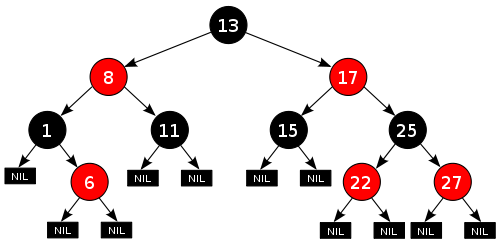
\includegraphics[scale=0.5]{rbtree.png}
  				\caption{Red-Black Tree}
  				\label{fig:ejemplo}
			\end{figure}
			
			\begin{center}
				\textbf{¿Cuantos BST ven en la imagen?}
			\end{center}
		\end{frame}

	\subsection{Operaciones basicas}

%------------------------------------------------

		\begin{frame}
			\frametitle{Operaciones basicas}
			Las principales operaciones de un BST son:
			\begin{itemize}[<+->]
				\item \textbf{Inserción}
				\item \textbf{Borrado}: No es necesaria para el sorting.
				\item \textbf{Búsqueda}: No es necesaria para el sorting.
				\item \textbf{Recorridos}:
					\begin{itemize}[<+->]
						\item EnOrden
						\item PostOrden
						\item PreOrden
					\end{itemize}
			\end{itemize}
		\end{frame}

		\begin{frame}
			\frametitle{El peor caso de inserción}
			\begin{figure}
  				\centering
    			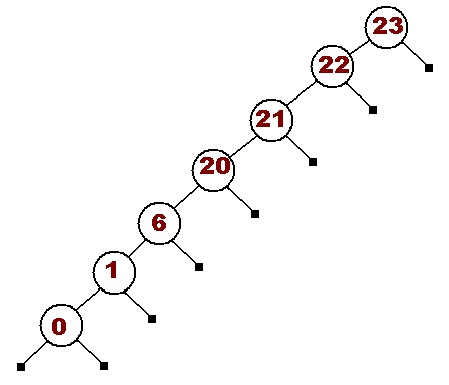
\includegraphics[scale=0.3]{lls.jpg}
  				\caption{Worst case evah!}
  				\label{fig:lls}
			\end{figure}
		
			\begin{center}
				\textbf{Para insertar -1 tendriamos que pasar por cada nodo!}
			\end{center}
		\end{frame}

		\begin{frame}
			\frametitle{Ejemplo de recorrido EnOrden}
			\begin{figure}
  				\centering
    			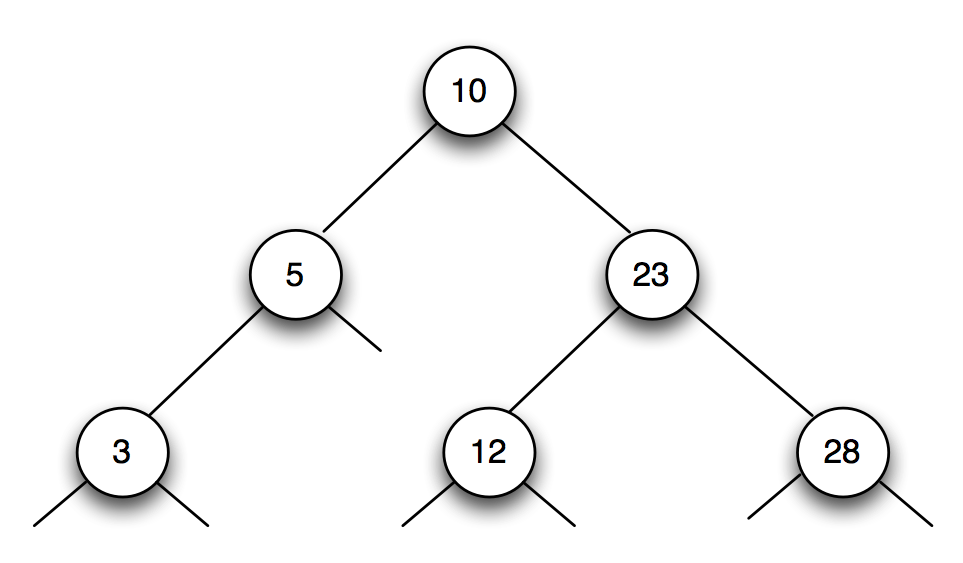
\includegraphics[scale=0.5]{inorden.png}
  				\caption{In-Orden}
  				\label{fig:inorden}
			\end{figure}
		
			\begin{center}
				El recorrido sería: [3-5-10-12-23-28]
			\end{center}
		\end{frame}
%------------------------------------------------
\section{BST Sort}
%------------------------------------------------

	\subsection{Uso del BST en el algoritmo}

		\begin{frame}
			\frametitle{Entonces ... ¿Que tiene que ver el bst con el ordenamiento?}
			Nos aprovechamos de la inserción y el recorrido EnOrden del arbol.
			\newline

			Al insertar en el arbol, los elementos son ordenados segun las reglas de este y al recorrerlo EnOrden son presentados de forma ordenada.
		\end{frame}

%------------------------------------------------

	\subsection{Complejidad y relación con la altura del árbol}

		\begin{frame}
			\frametitle{Complejidad y relación con la altura del árbol}
			En base al árbol podemos postular que su altura esta expresada en la siguiente formula:
				\begin{equation}
					n < = 2^{(h + 1)} - 1
				\end{equation}
				Obteniendo que:
				\begin{equation}
					h >= \log_2{(n)}
				\end{equation}
				
			Esta es la característica principal de un árbol, la que permite que las operaciones sean tan rápidas, el único inconveniente es asegurar este mínimo valor para la altura ...
		\end{frame}

		\subsection{El algoritmo en si}

			\begin{frame}
				\frametitle{Codigo}
				\lstinputlisting[language=Python, firstline=7, scale=0.5]{../bstsort.py}
			\end{frame}

\section{Conclusiones}

	\begin{frame}
		\frametitle{Conclusiones}
			\begin{itemize}[<+->]
				\item Se puede mejorar usando arboles autobalanceables, aunque estar asegurando minuciosamente puede añadir un costo considerable.
				\item No se nota la tendencia logaritmica de las inserciones debido a la complejidad lineal del recorrido.
			\end{itemize}
	\end{frame}

\end{document} 
